\section{Casi D'uso}
\begin{figure}[H]
    \centering
    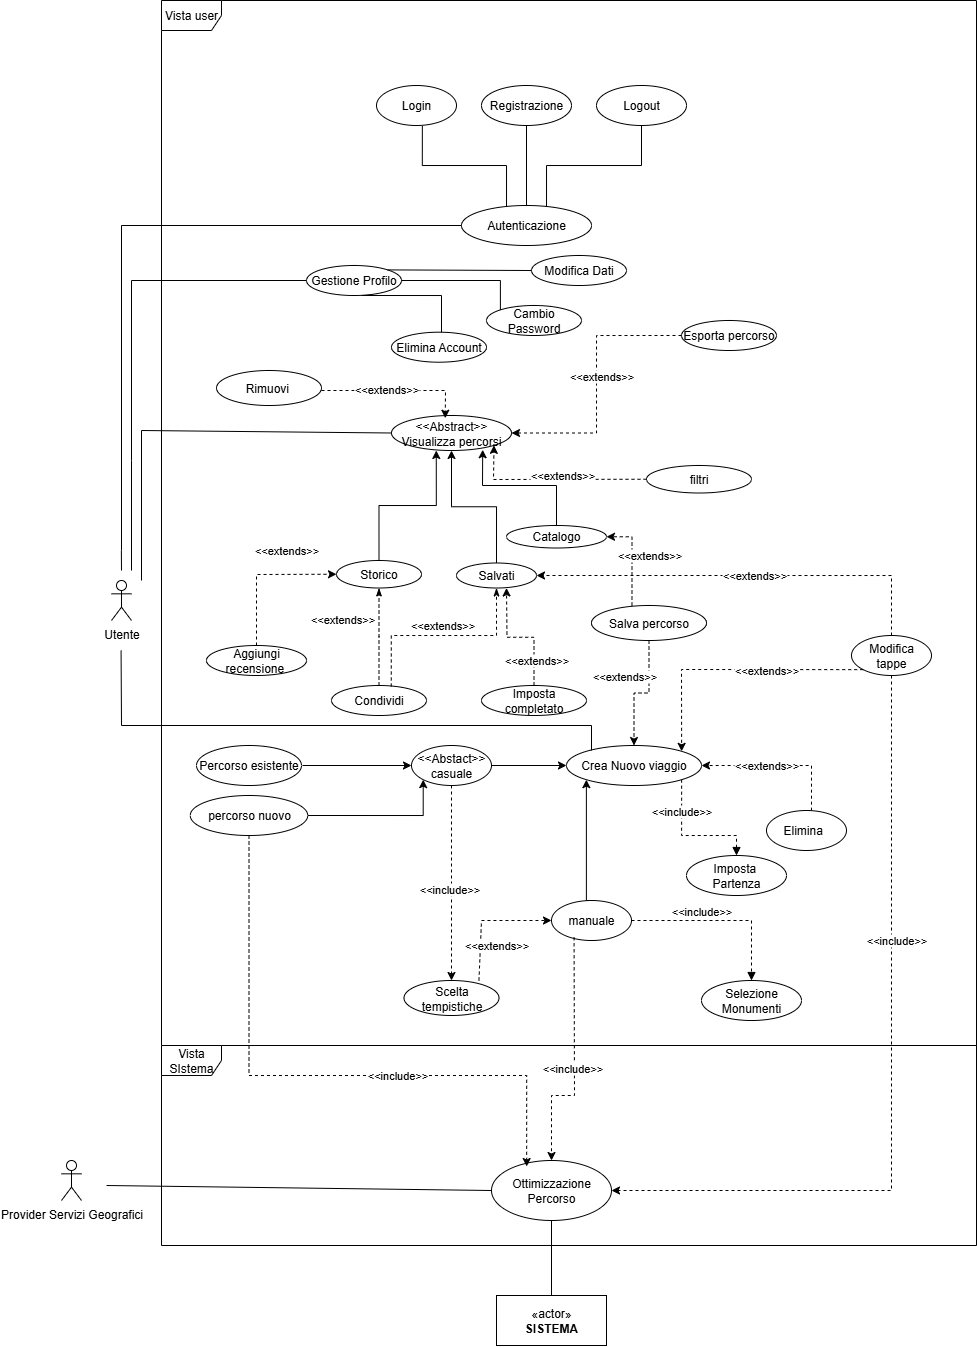
\includegraphics[width=0.8\textwidth]{Iterazione0/Diagrammi/DiagrammaCasiDusoV1.png}
    \caption{Casi d'uso}
    \label{fig:casi_d_uso}
\end{figure}    

Di seguito sono riportati i casi d’uso relativi al sistema di gestione percorsi e viaggi.
\begin{itemize}
  
    \item \textbf{UC1 - Autenticazione} 
 \begin{itemize}
  \item \textbf{UC1.1 - Registrazione:} un nuovo utente può creare un account personale fornendo i dati richiesti.

    \item \textbf{UC1.2 - Login:} un utente registrato può accedere al proprio account inserendo le proprie credenziali per iniziare una sessione e usare le funzionalità del sistema.

    \item \textbf{UC1.3 - Logout:} l’utente può terminare la propria sessione in modo sicuro.
\end{itemize}
    \item \textbf{UC2 - Gestione profilo}\begin{itemize}
   \item \textbf{UC2.1 - Modifica dati:} l'utente può modificare i propri dati personali in caso di neccessità.
    \item \textbf{UC2.2 - Elimina account:} l'utente può eliminare definitivamente il proprio account.
\end{itemize}


    \item \textbf{UC3 - Visualizza percorsi:} l'utente può visualizzare i dettagli di un percorso.
\begin{itemize}
    \item \textbf{UC3.1 - Catalogo:} è possibile visualizzare percorsi creati da altri utenti e inseriti in un catalogo.
    \item \textbf{UC3.2 - Salvati:} è possibile visualizzare percorsi provenienti dall’elenco dei percorsi salvati.
    \item \textbf{UC3.3 - Storico:} è possibile visualizzare percorsi provenienti dallo storico dei percorsi effettuati.
\end{itemize}

    \item \textbf{UC4 - Filtri ricerca:} l'utente può filtrare i percorsi in base a diversi criteri.

    \item \textbf{UC5 - Salva percorso:} l'utente può salvare un percorso nella sezione dei percorsi preferiti.

    \item \textbf{UC6 - Esporta percorso:} l'utente può esportare un percorso in un formato condivisibile.

    \item \textbf{UC7 - Rimuovi percorso salvato:} l'utente può rimuovere un percorso dai percorsi salvati.

    \item \textbf{UC8 - Condividi percorso:} l'utente può condividere un percorso con altri utenti.

    \item \textbf{UC9 - Aggiungi recensione:} l'utente può aggiungere una recensione a un percorso che è satao effettuato.

    \item \textbf{UC10 - Imposta percorso completato:} l'utente può contrassegnare un percorso come completato.

    \item \textbf{UC11 - Imposta punto di partenza:} l'utente seleziona il punto da cui far partire e finire il percorso.

    \item \textbf{UC12 - Crea nuovo viaggio:} 
\begin{itemize}
     \item \textbf{UC12.1 - Manuale:} l'utente può far creare il proprio percorso scegliendo autonomamente le tappe da visitare.
 \item \textbf{UC12.2 - Casuale:} 
\begin{itemize}
   \item \textbf{UC12.2.1 - Percorso esistente:} l'utente fa scegliere al sistema in modo casuale un percorso già esistente nel catalogo.
    \item \textbf{UC12.2.2 - Percorso nuovo:} l'utente fa generare al sistema in modo casuale un nuovo percorso.
\end{itemize}
\end{itemize} 

    \item \textbf{UC13 - Scelta tempistiche:} l'utente può definire le tempistiche del viaggio.

    \item \textbf{UC14 - Ottimizzazione percorso:} il sistema ottimizza tramite un algoritmo specifico l’ordine delle tappe.

    \item \textbf{UC15 - Modifica tappe:} l'utente può modificare le tappe di un percorso.

    \item \textbf{UC16 - Elimina tappa:} l'utente può eliminare una tappa dal percorso.
\end{itemize}